\documentclass[a4paper,12pt]{article}

\title{Biology 30 IB \\ Cells, Chromosomes, \& DNA}
\author{Jad Chehimi}

% document setup
\renewcommand{\familydefault}{\sfdefault}
\linespread{1.25}
\usepackage[margin=1in]{geometry}
\usepackage{setspace}
\usepackage{enumitem}
\setlist{nosep}
\usepackage{amsmath}
\usepackage{color,soul}
\setcounter{secnumdepth}{0}
\usepackage{wasysym}

% tools
\usepackage[hidelinks]{hyperref}
\usepackage{float}
%% images
\usepackage{graphicx}
\graphicspath{ {./images/} }
%% science
\usepackage{siunitx}

\begin{document}
\maketitle

% temp
\begin{center}
\Huge
Unfinished!
\normalsize
\end{center}
% temp

\tableofcontents

\pagebreak

\section{Terms}
\begin{itemize}
    \item{\textbf{Somatic cells} are all cells in the body \hl{except sex cells} --- sperm and egg cells}
    \item{A human somatic cell has \hl{46 chromosomes}}
    \item{\textbf{Cell division} is done by Eukaryotic cells --- have a nucleus}
    \item{\textbf{Binary fission} is done by Prokaryotic cells --- have no nucleus, such as \hl{bacteria}}
\end{itemize}

\section{Cell Division}
\subsection{Purpose}
\begin{itemize}
    \item{Unicellular organisms (i.e. \hl{zygote}) $\longrightarrow$ Multicellular organisms}
    \item{Growth and maintenance of body cells --- \hl{replacement} of worn out cells}
\end{itemize}

\subsection{Chromosomes}
\begin{itemize}
    \item{
            Comprised of...
            \begin{itemize}
                \item{nucleic acids (DNA)}
                \item{proteins}
            \end{itemize}
        }
    \item{
            Either...
            \begin{itemize}
                \item{\textbf{Uncondensed} aka. \textbf{Chromatin} = long, thin strands. invisible to microscope}
                \item{\textbf{Condensed} = thick \& shortened. visible to microscope}
            \end{itemize}
        }
\end{itemize}

\subsection{Chromatid}
\begin{itemize}
    \item{The strand that makes up a normal chromosome}
    \item{
            In mitosis...
            \begin{itemize}
                \item{A chromosome duplicates into two \hl{identical} chromatids, joined together by a \textbf{centromere}, to form a \textbf{duplicated chromosome}}
                \item{These chromatids are referred as \textbf{sister chromatids} in this state}
                \item{Each chromatid of a duplicated chromosome goes to each of the two new cells}
            \end{itemize}
        }
\end{itemize}

\begin{figure}[H] 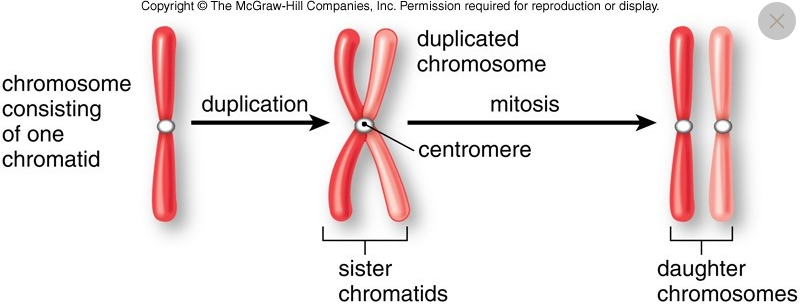
\includegraphics[width=\textwidth]{chromosome} \end{figure}

\section{Cell Cycle}
\begin{figure}[H] 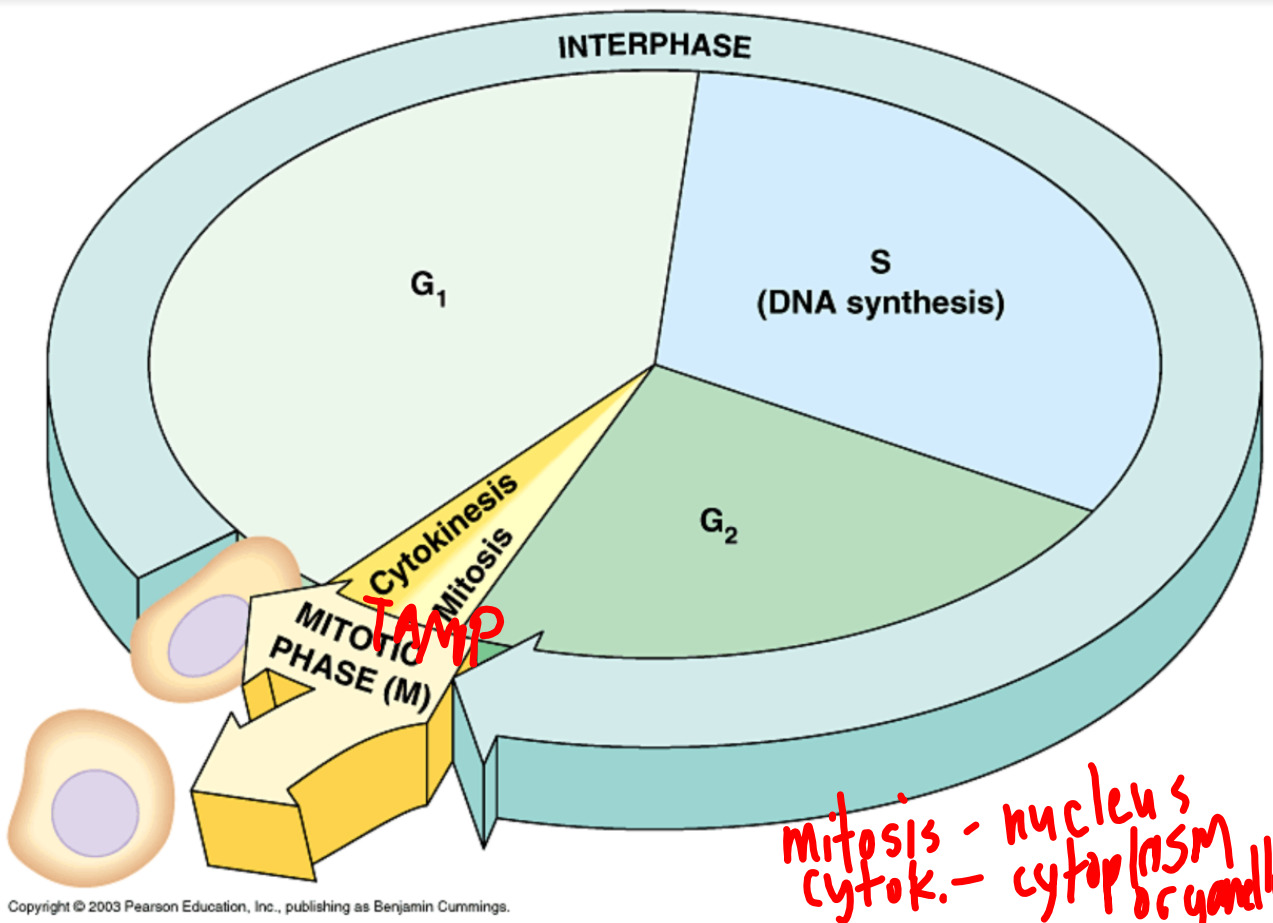
\includegraphics[width=\textwidth]{cellcycle} \end{figure}

A continuous cycle that involves all steps of a cell's life, especially cell division.

\subsection{Interphase}

\begin{itemize}
    \item{90\% of cell cycle}
    \item{All cell activity when not dividing}
\end{itemize}

\subsubsection{Gap 1 ($G_1$)}
\begin{itemize}
    \item{Cell growth and general function}
    \item{After cell division, cells may be smaller than their parent. Cell growth is needed}
\end{itemize}

\subsubsection{S Phase ($S$)}
\begin{itemize}
    \item{DNA is doubled}
    \item{Single(-chromatid) chromosome $\xrightarrow{\textrm{duplication}}$ double(-chromatid) chromosome}
\end{itemize}

\subsubsection{Gap 2 ($G_2$)}
\begin{itemize}
    \item{Organelles are doubled, and proteins for the new cell are produced}
\end{itemize}

\pagebreak

\subsection{Mitotic Phase}\noindent

Occurs in somatic cells.

Distribution of \hl{nucleus and its contents}.

\subsubsection{Prophase}
\begin{itemize}
    \item{Chromatin condense --- shorten \& thicken --- into chromosomes, becoming visible}
    \item{Nuclear membrane fades}
    \item{
            Animal cells only...
            \begin{itemize}
                \item{\textbf{Centrioles} (aka. centrosomes) move to opposite poles of cell. (N/S, E/W)}
                \item{Two centrioles are at each pole, total four, for each cell}
                \item{Centrioles deploy \textbf{spindle fibers}}
            \end{itemize}
        }
    \item{Without centrioles --- such as plant cells --- spindle fibers are still present and the cycle works the same}
\end{itemize}

\begin{figure}[H]
    \centering
    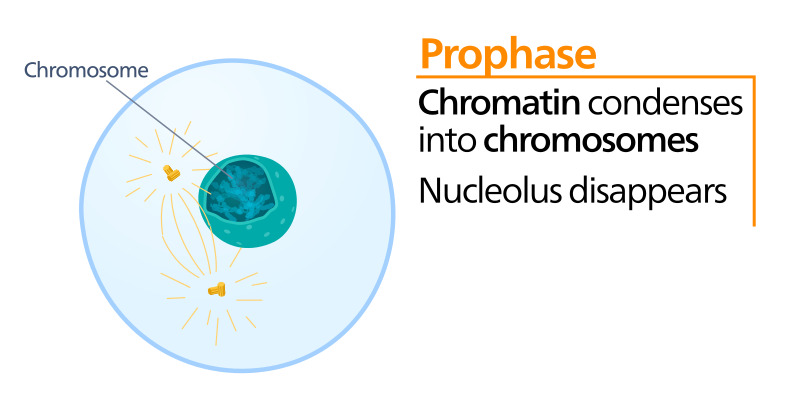
\includegraphics[width=0.5\textwidth]{prophase}
\end{figure}

\subsubsection{Metaphase}
\begin{itemize}
    \item{\textbf{Equatorial plate} = center of cell}
    \item{Sister chromatids move towards equatorial plate}
    \item{Chromosomes attach to spindle fibers}
\end{itemize}

\begin{figure}[H]
    \centering
    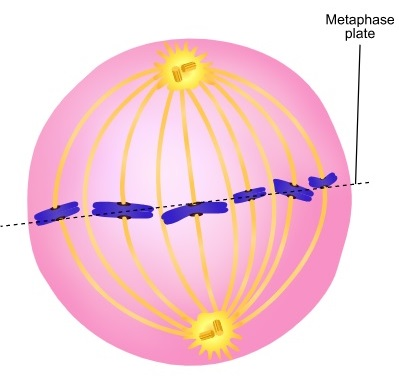
\includegraphics[width=0.5\textwidth]{metaphase}
\end{figure}

\pagebreak

\subsubsection{Anaphase}
\begin{itemize}
    \item{Centromeres divide}
    \item{(Now) chromatids move towards spindle fibers --- i.e. opposite poles of cell}
\end{itemize}

\begin{figure}[H]
    \centering
    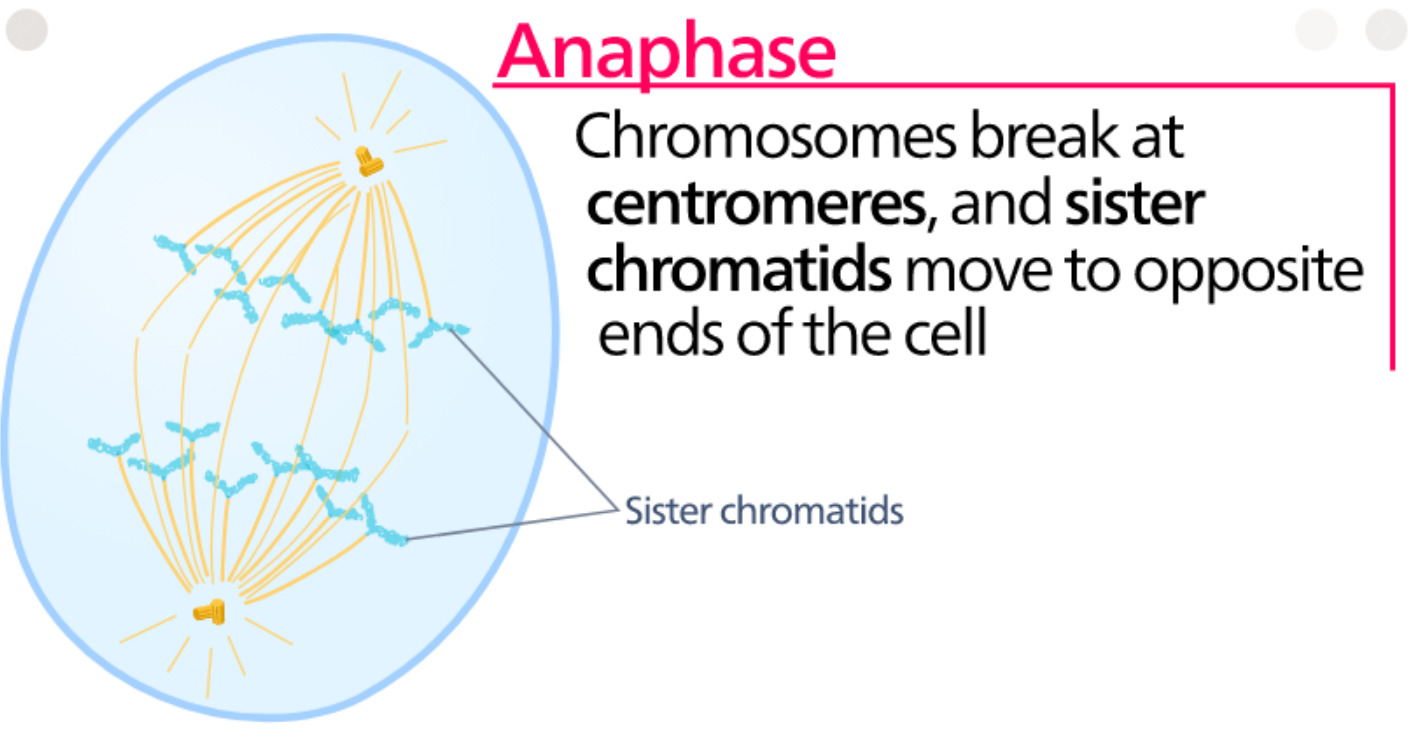
\includegraphics[width=0.75\textwidth]{anaphase}
\end{figure}

\subsubsection{Telophase}
\begin{itemize}
    \item{Spindle fibers dissolve}
    \item{Nuclear membrane forms around each mass of chromatin}
\end{itemize}

\subsubsection{Cytokinesis}
Technically occurs at the end of telophase.
\begin{itemize}
    \item{\hl{Division of cytoplasm} and \hl{distribution of organelles} to "daughter" cells}
    \item{Involves \textbf{cleavage}, pinching off in the center as the cytoplasm moves to opposite poles}
    \item{In plant cells only, a \textbf{cell plate} is distributed, which develops into a new cell wall}
\end{itemize}

\begin{figure}[H]
    \centering
    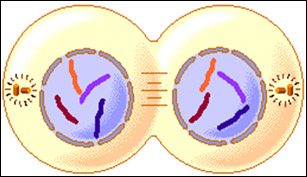
\includegraphics[width=0.75\textwidth]{telophase}
\end{figure}

\section{Cell Properties}

\subsection{Biological Clock}\noindent

Immature cells always have \hl{50 division}, regardless of...
\begin{itemize}
    \item{duration frozen}
    \item{stage/phase that cell division was suspended}
\end{itemize}

\subsection{Death \& Aging}\noindent

Cells may stop dividing due to...
\begin{itemize}
    \item{\textbf{Senescence} = aging, irreversible changes that eventually lead to death}
    \item{\textbf{Specialization} = the more \hl{specialized/differentiated} a cell is, the less likely it will undergo mitosis}
\end{itemize}

Cells that avoid aging are...
\begin{itemize}
    \item{\textbf{Spermatogonia} = sperm-producing cells, immature \& unspecialized}
    \item{Cancer cells of a tumor, which do not become specialized}
\end{itemize}

\section{Natural Cloning}
\begin{itemize}
    \item{Asexual/nonsexual reproduction}
    \item{Identical offspring from a single cell}
\end{itemize}

\subsection{Twins}
\begin{figure}[H]
    \centering
    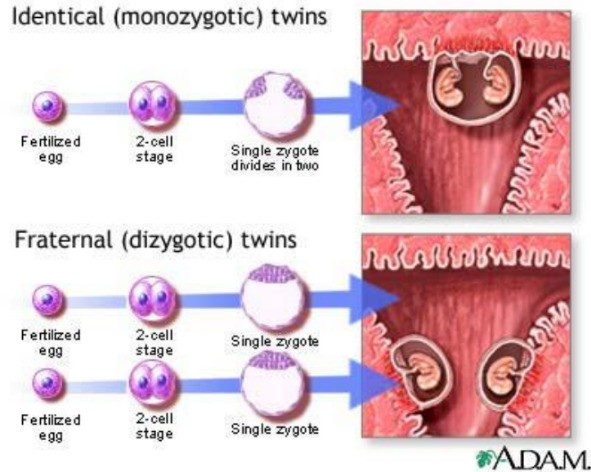
\includegraphics[width=0.9\textwidth]{twins}
\end{figure}

\subsection{Identical Twins}
\begin{itemize}
    \item{Originate from single egg cell}
    \item{During mitosis, \hl{one of the cells breaks free}; this cell forms a 2nd embryo}
    \item{If cell clusters remain separate, two babies with identical gene structures will develop}
    \item{Same gender, blood type, similar facial structure (nature vs. nurture)}
\end{itemize}

\subsection{Fraternal Twins}
\begin{itemize}
    \item{Two different eggs fertilized by different sperm cells}
    \item{Not to be confused with identical twins --- do not have identical genes}
\end{itemize}

\pagebreak

\section{Unnatural Cloning}

A \textbf{totipotent} nucleus is a nucleus that is able to bring a cell from \hl{egg to adult}.

\subsection{Plant Cloning}
\begin{itemize}
    \item{useful, since cloned plants have predictable characteristics}
    \item{requires \hl{delaying cell specialization}}
\end{itemize}

\subsection{Animal Cloning}
\begin{itemize}
    \item{With a micropipette, the nucleus is extracted from an unfertilized egg cell\\The cell is now \textbf{enucleated} (no nucleus)}
    \item{Remove nucleus from a cell of another frog}
    \item{Insert egg cell nucleus into said cell}
    \item{If cell is in \textbf{blastula} stage --- hollow ball of cells of an embryo, early embryo --- then the cells divide into an adult frog, a clone of the frog that donated the \hl{egg cell nucleus}}
    \item{If cell is past blastula --- such as the later \textbf{gastrula} stage --- the cells have \hl{already specialized}, so they do not divide, and the embryo dies}
\end{itemize}

\begin{figure}[H]
    \centering
    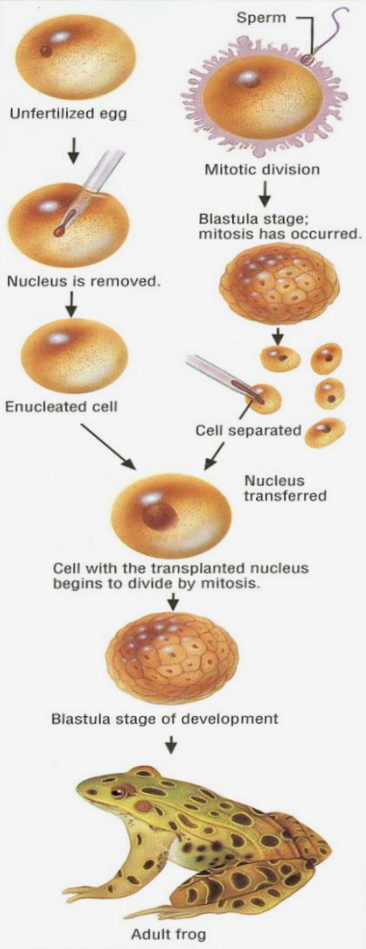
\includegraphics[width=0.3\textwidth]{clone}
\end{figure}

\subsubsection{Mammal Cloning}
\begin{itemize}
    \item{More difficult}
    \item{Cells tend to be \hl{more specialized}}
    \item{Nucleus transfer must be done before 8 cell stage of development}
    \item{Ensures nuclei are totipotent}
    \item{Needs \textbf{surrogate} --- implanting an embryo into a surrogate and having the surrogate birth the offspring. No genetics from surrogate transfer.}
\end{itemize}

\begin{figure}[H]
    \centering
    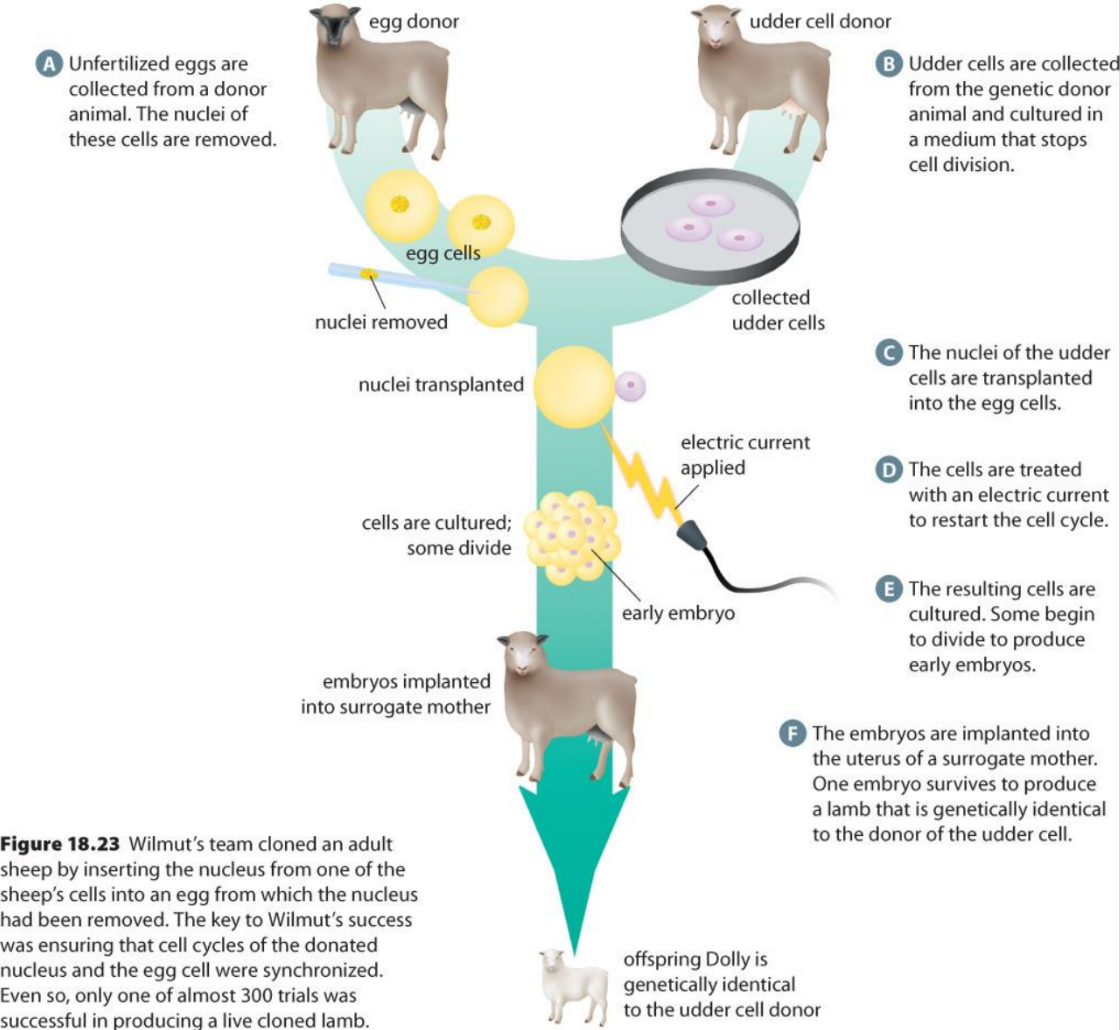
\includegraphics[width=\textwidth]{clone2}
\end{figure}

\pagebreak

\section{Cancer}
\begin{itemize}
    \item{Rapid, uncontrollable growth of cells}
    \item{\hl{Divide faster than normal cells}}
    \item{Some are very slow, some pause and return after many years}
    \item{\hl{Reproduce without directions} from adjacent cells}
    \item{\hl{Cannot specialize} --- making them inefficient}
\end{itemize}

\subsection{Metastasis}
\begin{itemize}
    \item{Cancer cells can dislodge from a tumor and \hl{move to another area}}
    \item{Difficult to isolate source of cancer}
\end{itemize}

\subsection{Tumors}\noindent

A mass of cancerous cells within otherwise normal tissue.

\begin{itemize}
    \item{
            \textbf{Benign Tumor}

            \begin{itemize}
                \item{If cancerous cells remain at site}
                \item{Do not cause serious problems}
                \item{Can be removed by surgery}
            \end{itemize}
        }
    \item{
            \textbf{Malignant Tumor}

            \begin{itemize}
                \item{If cancerous cells metastasize --- dislodge \& travel --- and cause \hl{impairment of other organs}}
                \item{Unusual number of chromosomes}
            \end{itemize}
        }
\end{itemize}

\subsection{Causes}
\begin{itemize}
    \item{x-rays}
    \item{chemical poisons}
    \item{asbestos}
    \item{fungi}
    \item{oncoviruses}
    \item{environmental factors (nature, e.g. diet)}
    \item{age}
    \item{inherited mutations}
\end{itemize}

\subsection{Methods of Identification}
\begin{itemize}
    \item{x-rays}
    \item{cell biopsies}
    \item{infrared technology}
\end{itemize}

\section{Telomeres}
\begin{itemize}
    \item{Caps at the end of chromosomes}
    \item{\hl{Reduce in length every cell cycle/division}}
    \item{Clones --- like Dolly --- inherit their parents telomere length, \hl{shortening their life span} compared to non-clones} 
\end{itemize}

\begin{figure}[H]
    \centering
    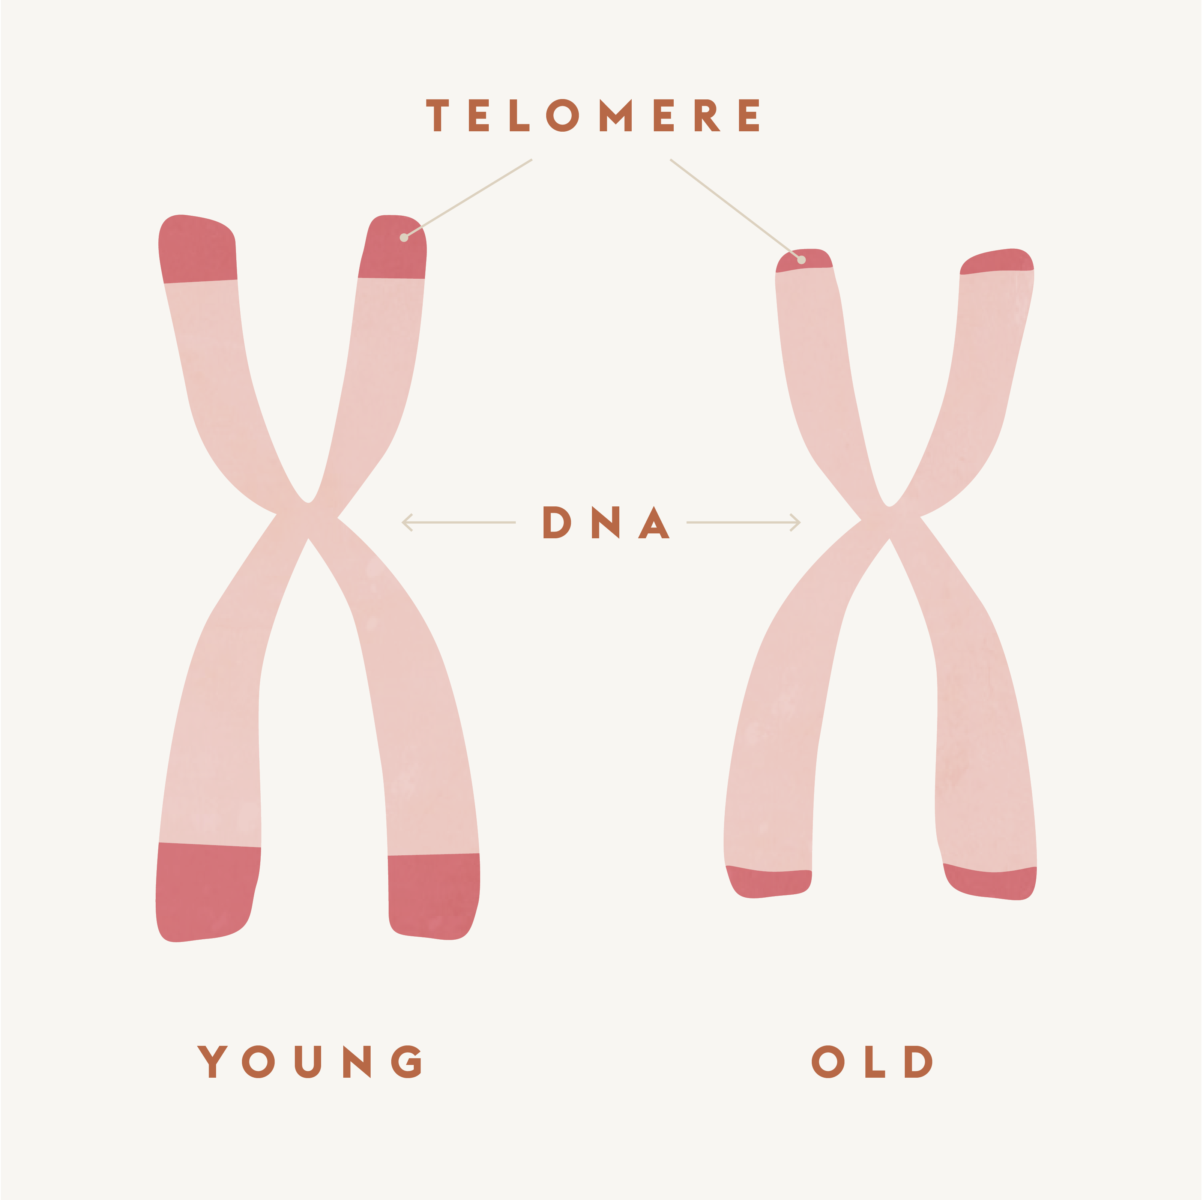
\includegraphics[width=0.50\textwidth]{telomere}
\end{figure}

\subsection{Telomerase}
\begin{itemize}
    \item{An enzyme that \hl{maintains telomere length}, slowing cell death}
    \item{Not present in most normal cells}
    \item{Reactivated in cancer cells, explaining their immortality}
\end{itemize}

\section{Sexual Cell Reproduction}

\subsection{Cons}
\begin{itemize}
    \item{consumes a lot of energy}
    \item{infections}
    \item{only half of the genes are passed (not necessarily a con)}
    \item{males are deadbeat --- contribute little to survival of offspring}
\end{itemize}

\subsection{Pros}
\begin{itemize}
    \item{Genetic diversity --- more potential for survival if environmental conditions change.}
    \item{
            Genetic diversity comes from...
            \begin{itemize}
                \item{independent assortment --- random shuffling and random order of genes in meiosis (metaphase I)}
                \item{crossing-over in meiosis (prophase I)}
                \item{random fertilization, combining genes of two separate individuals}
            \end{itemize}
        }
    \item{Two sets of chromosomes, so any damaged DNA has a \hl{backup}, and a \hl{template} to base \hl{DNA repairs} off of}
\end{itemize}

\section{Meiosis}
\begin{itemize}
    \item{\textbf{Gametes} = sex cells --- \female\! ova/ovum (eggs) and \male\! sperm cells}
    \item{\textbf{Gonads} = reproductive organs --- cells of \female\! ovaries and \male\! testes}
    \item{\textbf{Meiosis} = the process of forming gametes}
    \item{\textbf{Autosomes} = chromosomes not directly influenced by sex}
        \\
    \item{\textbf{Diploid} ($2n$) = cell --- such as \hl{somatic cells} --- with a typical \# of chromosomes, such as \hl{46 chromosomes in a human cell}}
    \item{\textbf{Haploid} ($n$) = cell --- such as \hl{gametes} --- with half the typical \# of chromosomes, such as \hl{23 chromosomes in a human gamete}}
\end{itemize}

Meiosis occurs in the germ cells of gonads.

\begin{figure}[H]
    \centering
    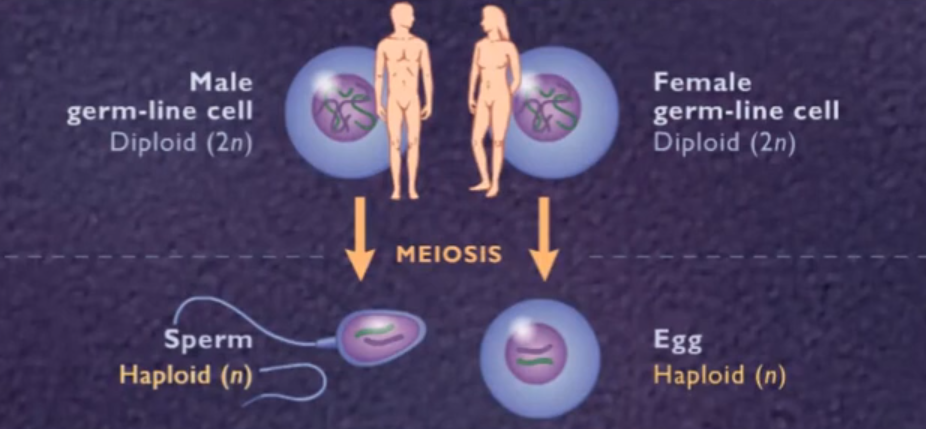
\includegraphics[width=\textwidth]{loid}
\end{figure}

\subsection{Composition of Cells}

\subsubsection{Gametes}
\begin{itemize}
    \item{22 autosomes}
    \item{
            1 sex chromosome
            \begin{itemize}
                \item{Ova can \hl{only} have \female X}
                \item{Sperm can have \hl{either} \female X or \male Y}
            \end{itemize}
        }
    \item{\hl{23 total chromosomes}}
\end{itemize}

\begin{figure}[H]
    \centering
    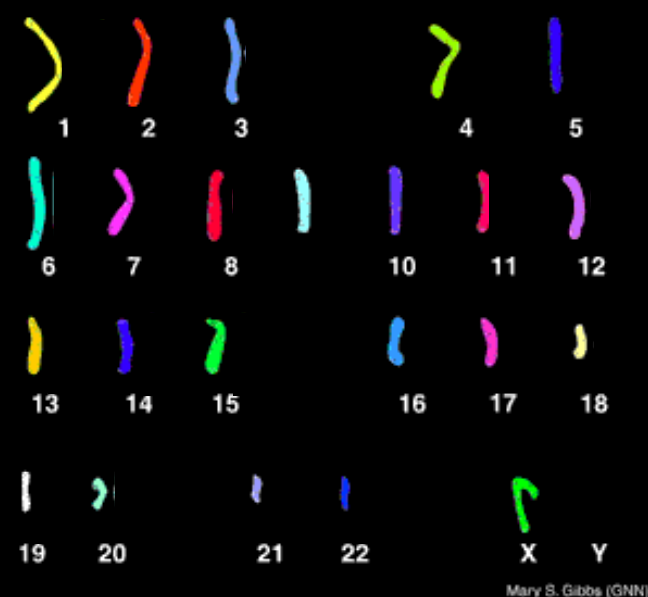
\includegraphics[width=0.45\textwidth]{23}
    \caption{If this were a sperm cell, and it fertilized an egg, the baby would be female}
\end{figure}

\subsubsection{Somatic}
\begin{itemize}
    \item{22 autosome \hl{pairs}}
    \item{2 sex chromosomes --- either \female XX or \male XY}
    \item{\hl{46 total chromosomes}}
\end{itemize}

\begin{figure}[H]
    \centering
    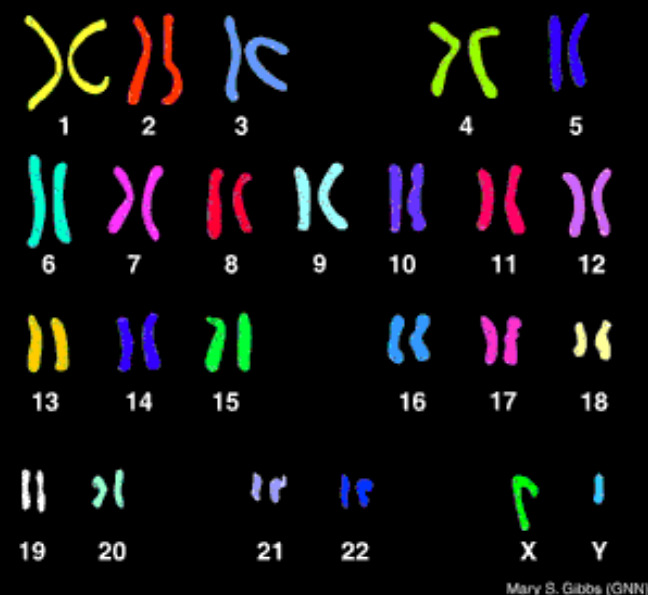
\includegraphics[width=0.45\textwidth]{46}
\end{figure}

\subsection{Union}
\begin{itemize}
    \item{\;\;\;\;23 chromosome (haploid) sperm cell from \male\! male}
    \item{+ 23 chromosome (haploid) egg cell \;\;\,\,\,from \female\! female}
    \item{= 43 chromosome (diploid) zygote or fertilized egg}
\end{itemize}

\section{Stages of Meiosis}

\subsection{Interphase (same as mitosis)}
\begin{itemize}
    \item{Not splitting}
    \item{Important part: S phase --- doubling 46 single chromosomes}
    \item{Ends up as 46 duplicated chromosomes (92 chromotids)}
\end{itemize}

\subsection{Meiosis I}

\subsubsection{Prophase I}
\begin{itemize}
    \item{Same beginning as mitosis
          \begin{itemize}
              \item{Nuclear membrane dissolves}
              \item{Centrioles move to opposite poles of cell, deploying spindle fibers}
          \end{itemize}
         }
     \item{\textbf{Homologous} = \hl{similar} --- such as shape, size, gene arrangement --- but \hl{not identical}}
     \item{Homologous chromosome pairs, one from the mother and one from the father, undergo \textbf{synapsis} --- pairing side by side}
     \item{This forms a \textbf{tetrad} --- 4 chromatids, homologous chromosome pair}
     \item{Chromosomes from the male and female \hl{shuffle around}, as well as \textbf{crossover}}
\end{itemize}
\textbf{Cross-Over}
\begin{itemize}
     \item{Inner chromatids of both chromosomes \textbf{cross-over} --- genetic recombination, exchange genetic information}
     \item{Chromatids of both chromosomes are \hl{no longer sister chromatids} after this point, \hl{not identical}}
\end{itemize}

\begin{figure}[H]
    \centering
    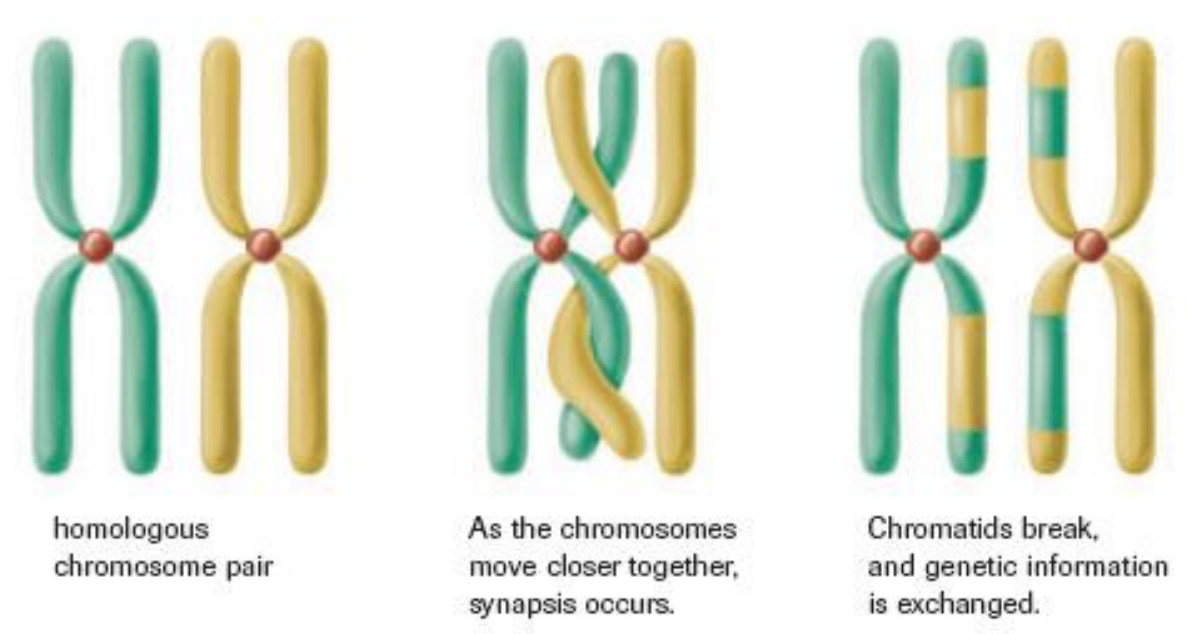
\includegraphics[width=0.6\textwidth]{synapsis}
\end{figure}

\subsubsection{Metaphase I (mostly same as mitosis)}
\begin{itemize}
    \item{Line up along equatorial plate, attach to spindle fibers}
    \item{Difference is instead of chromosomes lining up, \hl{tetrads line up}}
\end{itemize}

\begin{figure}[H]
    \centering
    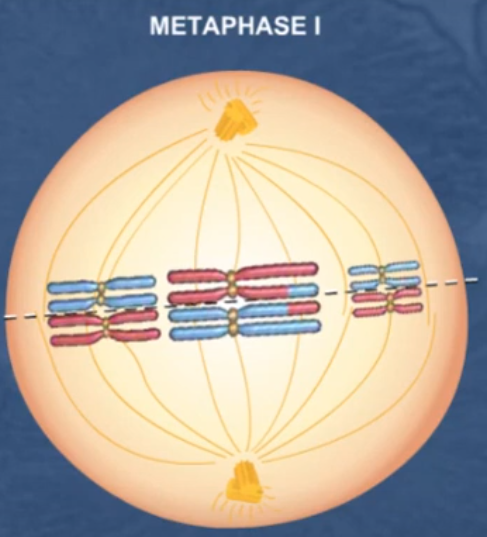
\includegraphics[width=0.4\textwidth]{metaphase-i}
\end{figure}

\subsubsection{Anaphase I (mostly same as mitosis)}
\begin{itemize}
    \item{Instead of splitting chromosomes, the homologous pairs are \textbf{segregated} (separated) and travel to opposite poles}
    \item{Diploid mother cell is now 2 haploid daughter cells}
\end{itemize}

\begin{figure}[H]
    \centering
    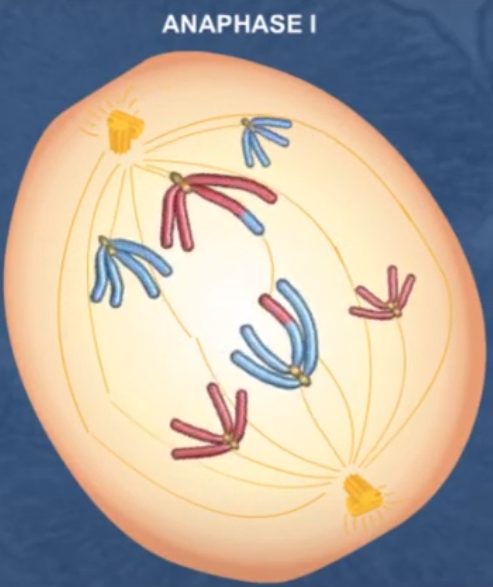
\includegraphics[width=0.4\textwidth]{anaphase-i}
\end{figure}

\subsubsection{Telophase I (same as mitosis)}
\begin{itemize}
    \item{
            The 2 cells are...
            \begin{itemize}
                \item{not identical to each other}
                \item{not identical to parent cell}
            \end{itemize}
        }
    \item{Each chromosome remains double stranded}
\end{itemize}

\subsection{Meiosis II}\noindent

Occurs at the same time in both of the daughter cells from Meiosis I.

No S phase.

\subsubsection{Same as Mitosis}
The following stages occur identically to mitosis.

\begin{itemize}
    \item{Prophase II}
    \item{Metaphase II}
    \item{Anaphase II}
    \item{Telophase II}
\end{itemize}

\subsection{Conclusion}
1 diploid mother somatic cell $\xrightarrow{\textrm{meiosis}}$ 4 haploid daughter gametes (sperm or egg)

\begin{figure}[H]
    \centering
    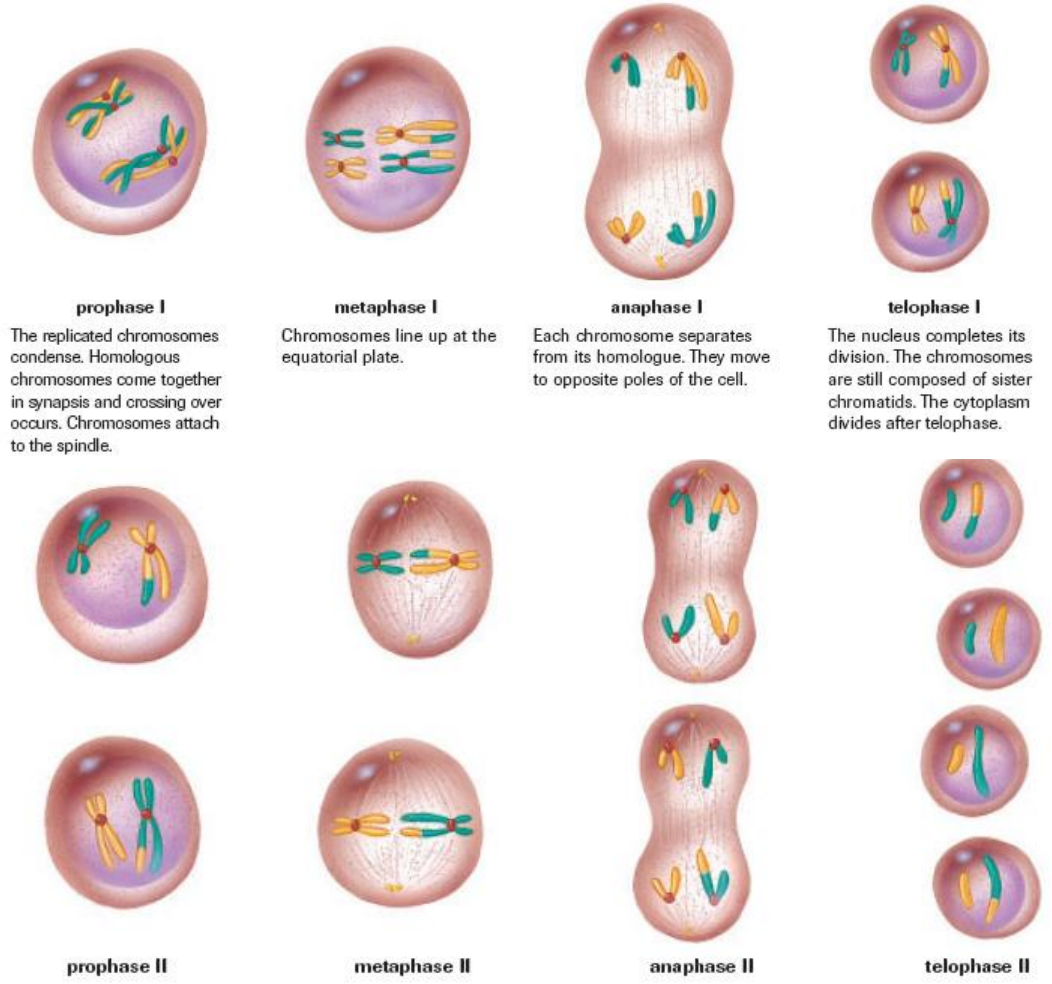
\includegraphics[width=0.9\textwidth]{meiosis}
\end{figure}

\section{Mitosis vs. Meiosis}
\begin{itemize}
    \item{\hl{Mitosis maintains} ploidy level (\# of chromosomes)}
    \item{\hl{Meiosis reduces} ploidy level}
        \\
    \item{Meiosis only occurs in gonad cells}
    \item{Mitosis is far more common}
\end{itemize}

\begin{figure}[H]
    \centering
    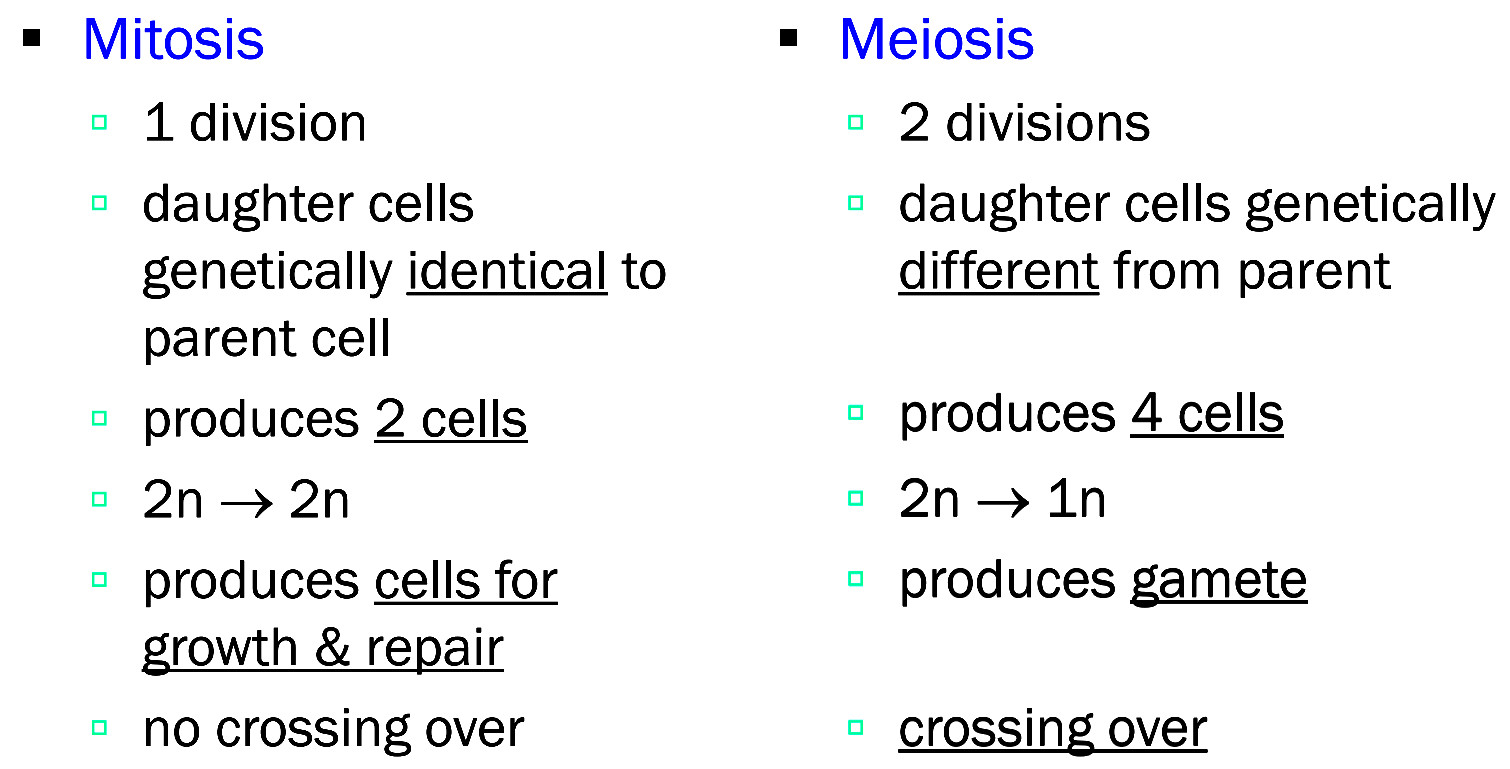
\includegraphics[width=\textwidth]{compare}
\end{figure}

\pagebreak

\section{Plant Sexual Reproduction}
\begin{itemize}
    \item{
            \textbf{Alternation of Generations}
            \begin{itemize}
                \item{plant sporophyte ($2n$) and gametophyte ($n$) take turns \hl{reproducing each other}}
            \end{itemize}
        }
    \item{Pollen are \male\! male sex cells}
    \item{\female\! Eggs are stored in a variety of locations}
    \item{Fertilization results in a seed}
\end{itemize}

\section{Development of \male\! Male and \female\! Female Gametes}
\begin{itemize}
    \item{\textbf{Gametogenesis} = formation of gametes during meiosis}
    \item{\textbf{Spermatogenesis} = formation of sperm cells}
    \item{
            \textbf{Spermatocyte} = a diploid cell that undergoes meiosis to become 4 sperm cells
            \begin{itemize}
                \item{Capable of many mitotic divisons before meiosis}
                \item{Explains males being able to produce 1 billion sperm per day}
            \end{itemize}
        }
\end{itemize}

\begin{figure}[H]
    \centering
    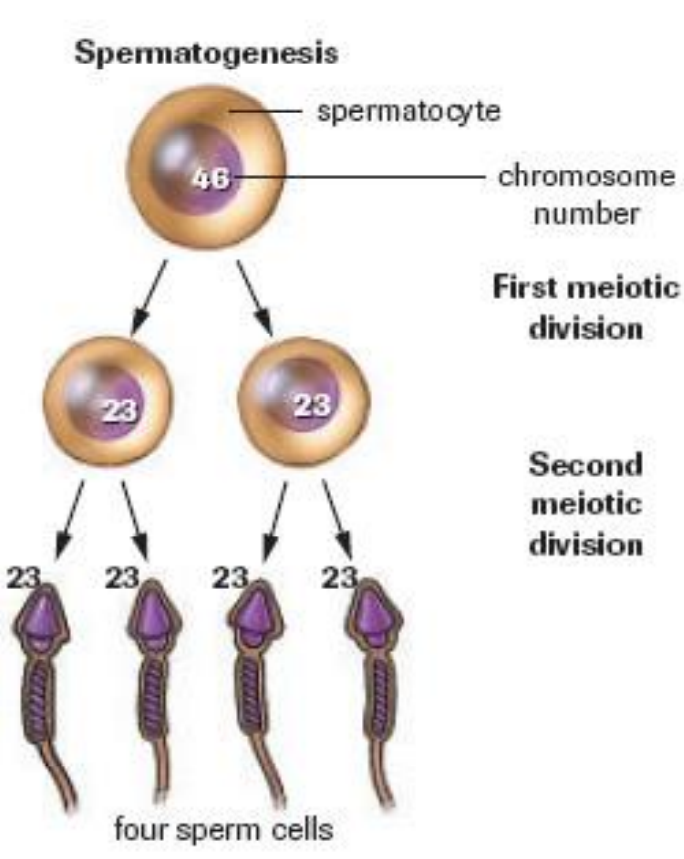
\includegraphics[width=0.7\textwidth]{spermatogenesis}
\end{figure}

\subsection{Oogenesis}
\begin{itemize}
    \item{Cytoplasm of female gametes (eggs) is \hl{not divided equally} after every division}
    \item{\textbf{Ootid} = The one daughter cell that recieves the most cytoplasm}
    \item{\textbf{Polar Body} = The other daughter cells die, their nutrients absorbed}
    \item{Only \hl{one egg is viable} for fertilization every division}
\end{itemize}

\begin{figure}[H]
    \centering
    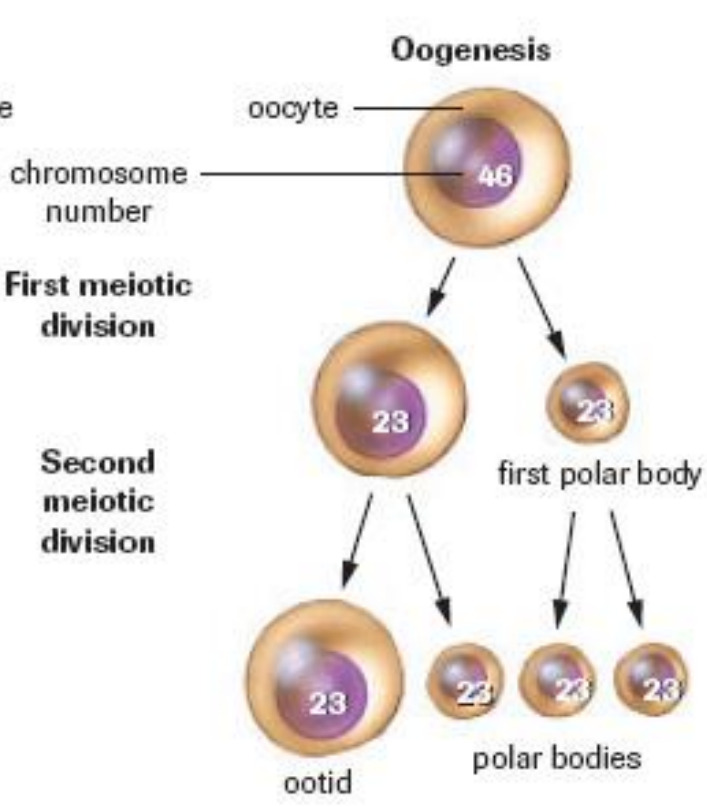
\includegraphics[width=0.4\textwidth]{oogenesis}
\end{figure}

\section{Immature $\longrightarrow$ Mature}
\begin{figure}[H]
    \centering
    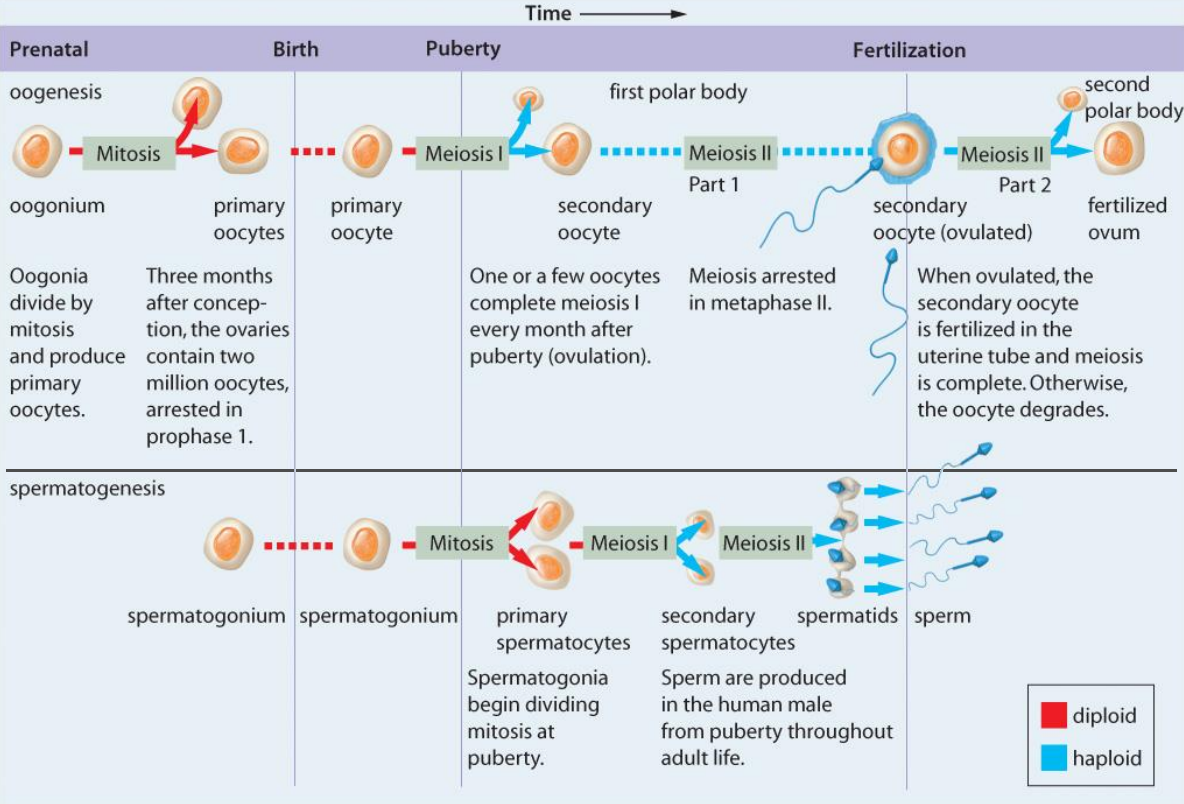
\includegraphics[width=\textwidth]{genesis}
\end{figure}

\section{Abnormal Meiosis}
Also known as \textbf{nondisjunction}.
\begin{itemize}
    \item{Occurs when 2 homologous chromosomes \hl{move to the same pole} during metaphase, meiosis or mitosis}
    \item{A cell will be missing a chromosome, and another will have an extra}
    \item{Cells with \hl{too much or too little} genetic information will \hl{not function correctly}}
\end{itemize}

\begin{figure}[H]
    \centering
    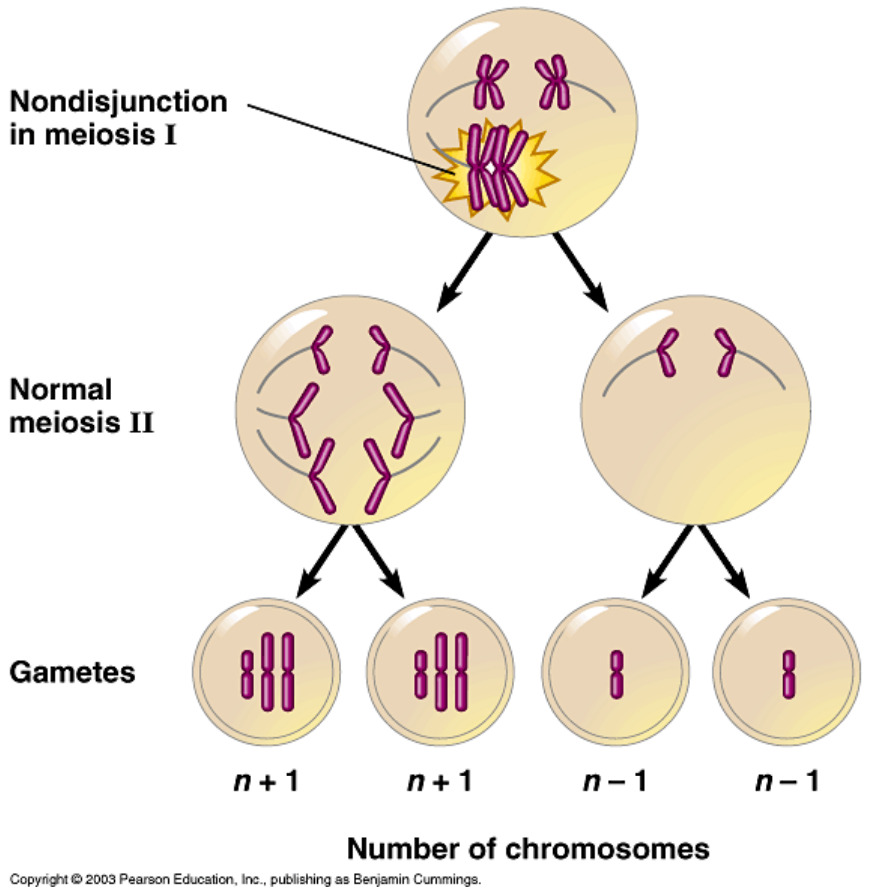
\includegraphics[width=0.6\textwidth]{nonj1}
\end{figure}

\begin{figure}[H]
    \centering
    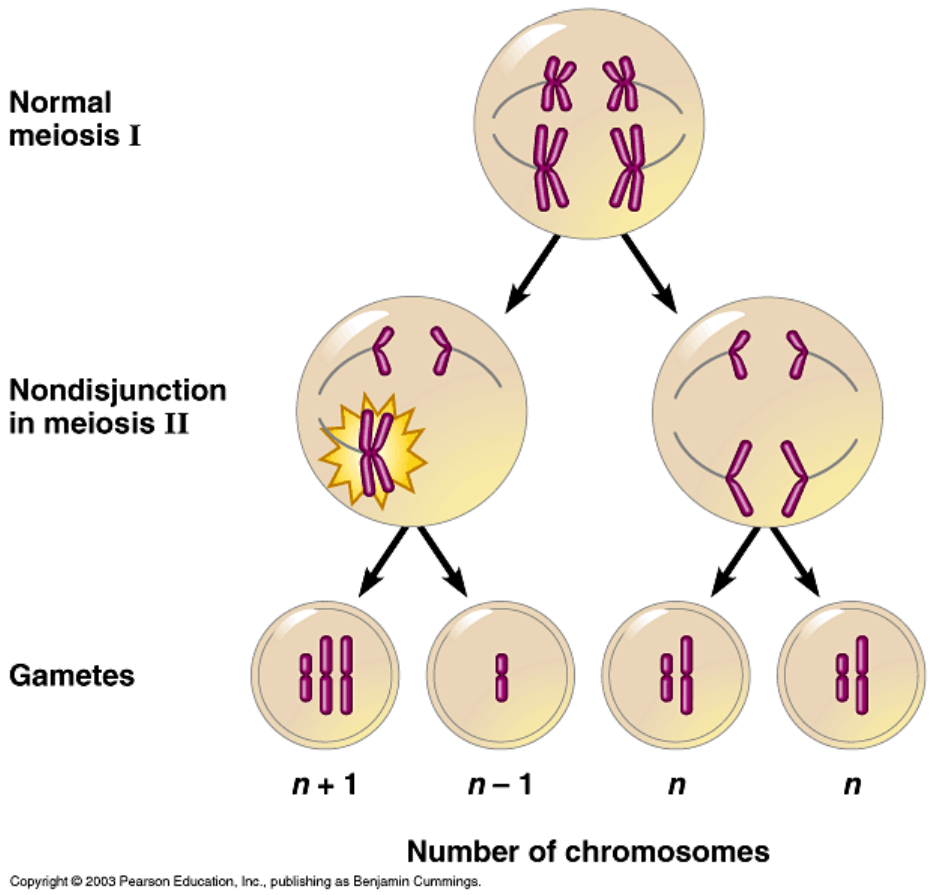
\includegraphics[width=0.6\textwidth]{nonj2}
\end{figure}

\subsection{Terms}
\begin{itemize}
    \item{\textbf{Karyotype chart} = A \hl{picture of chromosomes}, arranged in homologous pairs}
    \item{
            \textbf{Polyploidy} = An organism with \hl{$>2$ complete sets of chromosomes}
            \begin{itemize}
                \item{\textbf{Triploidy} ($3n$) = may result from abnormally diploid ($2n$) egg fertilized by normal ($n$) sperm, or vice versa}
                \item{\textbf{Tetraploidy} ($4n$) = doesn't occur in humans, failure of diploid zygote to divide after duplicating chromosomes following mitosis}
                \item{\textbf{Aneuploidy} = \hl{all cells} of the body contain \hl{abnormal \# of chromosomes}}
            \end{itemize}
        }
    \item{\textbf{Trisomy} = fertilized egg with \hl{3} \# of a chromosome (\hl{normally 2}) \\ normal gamete (23 pairs) + abnormal gamete (24 pairs), 47 chromosomes total}
    \item{\textbf{Monosomy} = fertilized egg with \hl{1} \# of a chromosome (\hl{normally 2}) \\ normal gamete (23 pairs) + abnormal gamete (22 pairs), 45 chromosomes total}
\end{itemize}

\subsection{Syndromes}

\subsubsection{Down Syndrome}
\begin{itemize}
    \item{\hl{Extra chromosome in pair \#21} (trisomic disorder)}
    \item{
            Causes...
            \begin{itemize}
                \item{mentally challenged}
                \item{round, full face}
                \item{enlarged, creased tongue}
                \item{short}
                \item{large forehead}
            \end{itemize}
        }
\end{itemize}

\subsubsection{Turner's Syndrome}
\begin{itemize}
    \item{\hl{Female with a single \female X chromosome (instead of \female XX)} (monosomic disorder)}
    \item{
            Causes...
            \begin{itemize}
                \item{no sexual development}
                \item{short}
                \item{thick, widened necks}
            \end{itemize}
        }
\end{itemize}

\subsubsection{Klinefelter Syndrome}
\begin{itemize}
    \item{\hl{Male with an extra \female X chromosome (XXY instead of XY)} (trisomic disorder)}
    \item{
            Causes...
            \begin{itemize}
                \item{high estrogen}
                \item{sterility}
            \end{itemize}
        }
\end{itemize}

\subsection{Teratogenic Compounds}
\begin{itemize}
    \item{Chemicals that cause abnormalities in embryos}
    \item{drugs (e.g. alcohol), infectious agents (viruses), radiation}
\end{itemize}

\section{Amniocentesis}
\begin{itemize}
    \item{Use of a syringe to \hl{draw fluid from sac} surrounding fetus}
    \item{Analysis can \hl{identify disorders}, \hl{down syndrome}, and \hl{sex}}
    \item{Amniotic fluid contains not a lot of cells from the fetus, so results take a while}
    \item{\textbf{Ultrasound} = used to locate position of fetus in womb}
        \\
    \item{\textbf{Chorionic Villus Sampling (CVS)} = draw cells from outer membrane surrounding embryo}
    \item{Can be \hl{done earlier and results quicker} than amniocentesis}
\end{itemize}

\begin{figure}[H]
    \centering
    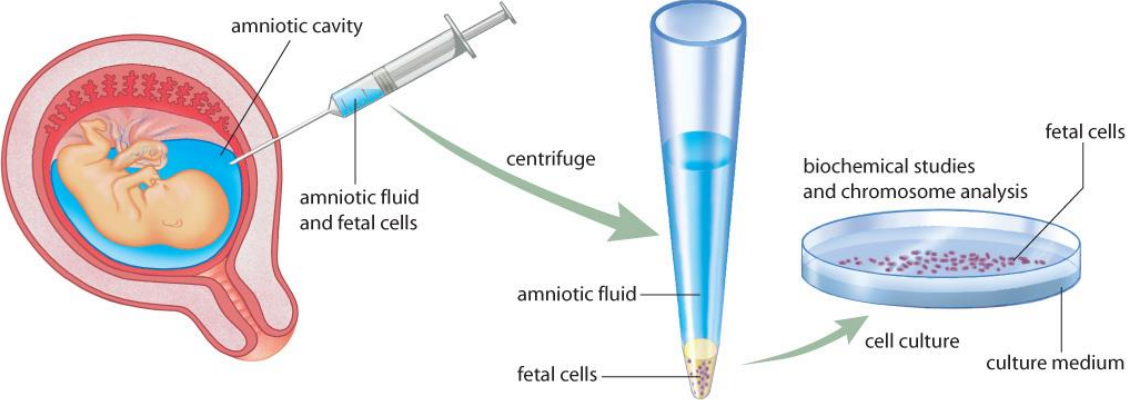
\includegraphics[width=\textwidth]{amnio}
\end{figure}

\end{document}
